\documentclass[tikz,border=0mm]{standalone}
\usepackage{tikz}
\usetikzlibrary{positioning}
\tikzset{
    mynodee/.style={minimum height=0mm, minimum width=0mm, inner sep=0mm
  },
  mynode/.style={
    draw, circle, minimum height=1.7mm, minimum  width=1.7mm,line width=0.5mm
  },
  rect/.style={
    draw, rectangle, rounded corners, minimum height=7mm, minimum  width=30mm,line
    width=0.5mm, dotted
  }
}

\begin{document}

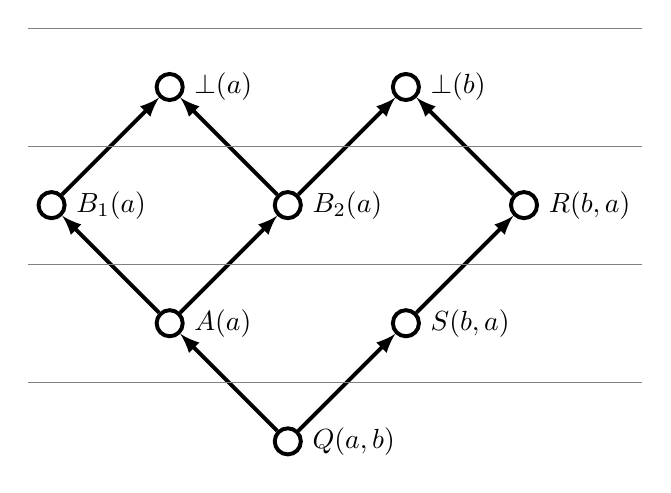
\begin{tikzpicture}
 \node[mynode, label=right:$\bot(a)$] (bota) at (0, 0) {};
 \node[mynode, label=right:$\bot(b)$] (botb) at (3, 0) {};
 \node[mynode, label=right:$B_1(a)$] (b1a) at (-1.5, -1.5) {};
 \node[mynode, label=right:$B_2(a)$] (b2a) at (1.5, -1.5) {};
 \node[mynode, label=right:{$R(b, a)$}] (rba) at (4.5, -1.5) {};
 \node[mynode, label=right:$A(a)$] (aa) at (0, -3) {};
 \node[mynode, label=right:{$S(b, a)$}] (sba) at (3, -3) {};
 \node[mynode, label=right:{$Q(a, b)$}] (qab) at (1.5, -4.5) {};

 \draw[-latex,line width=0.5mm] (b1a) -- (bota);
 \draw[-latex,line width=0.5mm] (b2a) -- (bota);
 \draw[-latex,line width=0.5mm] (b2a) -- (botb);
 \draw[-latex,line width=0.5mm] (rba) -- (botb);
 \draw[-latex,line width=0.5mm] (aa) -- (b1a);
 \draw[-latex,line width=0.5mm] (aa) -- (b2a);
 \draw[-latex,line width=0.5mm] (sba) -- (rba);
 \draw[-latex,line width=0.5mm] (qab) -- (aa);
 \draw[-latex,line width=0.5mm] (qab) -- (sba);
 \foreach \i in {0.75, -0.75, -2.25, -3.75} {
   \draw[very thin,gray] (-1.8, \i) -- (6, \i);
  }

\end{tikzpicture}

\end{document}

%%% Local Variables:
%%% mode: latex
%%% TeX-master: "fig-dllite"
%%% End:


